\section{Memory Efficiency and Training Performance}\label{sec:time_reduction}

\subsection{Memory Utilization}
Our layer-wise FP8 approach demonstrates significant memory savings, particularly at the 3B model scale. Table~\ref{tab:memory_results} presents memory utilization across different model scales and precision configurations.

\begin{table}[h]
\centering
\begin{tabular}{lccc}
\toprule
\textbf{Model} & \textbf{Precision} & \textbf{VRAM (GB)} & \textbf{Time (hours)} \\
\midrule
\multirow{3}{*}{Llama-3.2-3B} & BF16 & 82.4 & 3.6 \\
 & Hybrid FP8 & 74.2 & 2.2 \\
 & Ours (Layer-wise FP8) & \textbf{74.2} & \textbf{2.1} \\
\midrule
\multirow{3}{*}{Llama-3.1-8B} & BF16 & 80.0 & 9.1 \\
 & Hybrid FP8 & 88.0 & 7.6 \\
 & Ours (Layer-wise FP8) & 88.3 & \textbf{6.6} \\
\bottomrule
\end{tabular}
\caption{Memory utilization and training time across model scales and precision formats.}
\label{tab:memory_results}
\end{table}

For Llama-3.2-3B, our approach achieves 10.0\% memory reduction (from 82.4 GB to 74.2 GB) compared to BF16 baseline, enabling larger batch sizes within the same hardware constraints. For Llama-3.1-8B, we observe higher allocated VRAM (88.3 GB vs 80.0 GB for BF16), likely due to workspace and scaling-metadata overheads in the current implementation.

\subsection{Training Time Performance}
Our layer-wise FP8 method delivers substantial training time improvements across both model scales. Figure~\ref{fig:training_time_comparison} illustrates the relative training time across different model configurations and precision formats.

\begin{figure}[h]
    \centering
    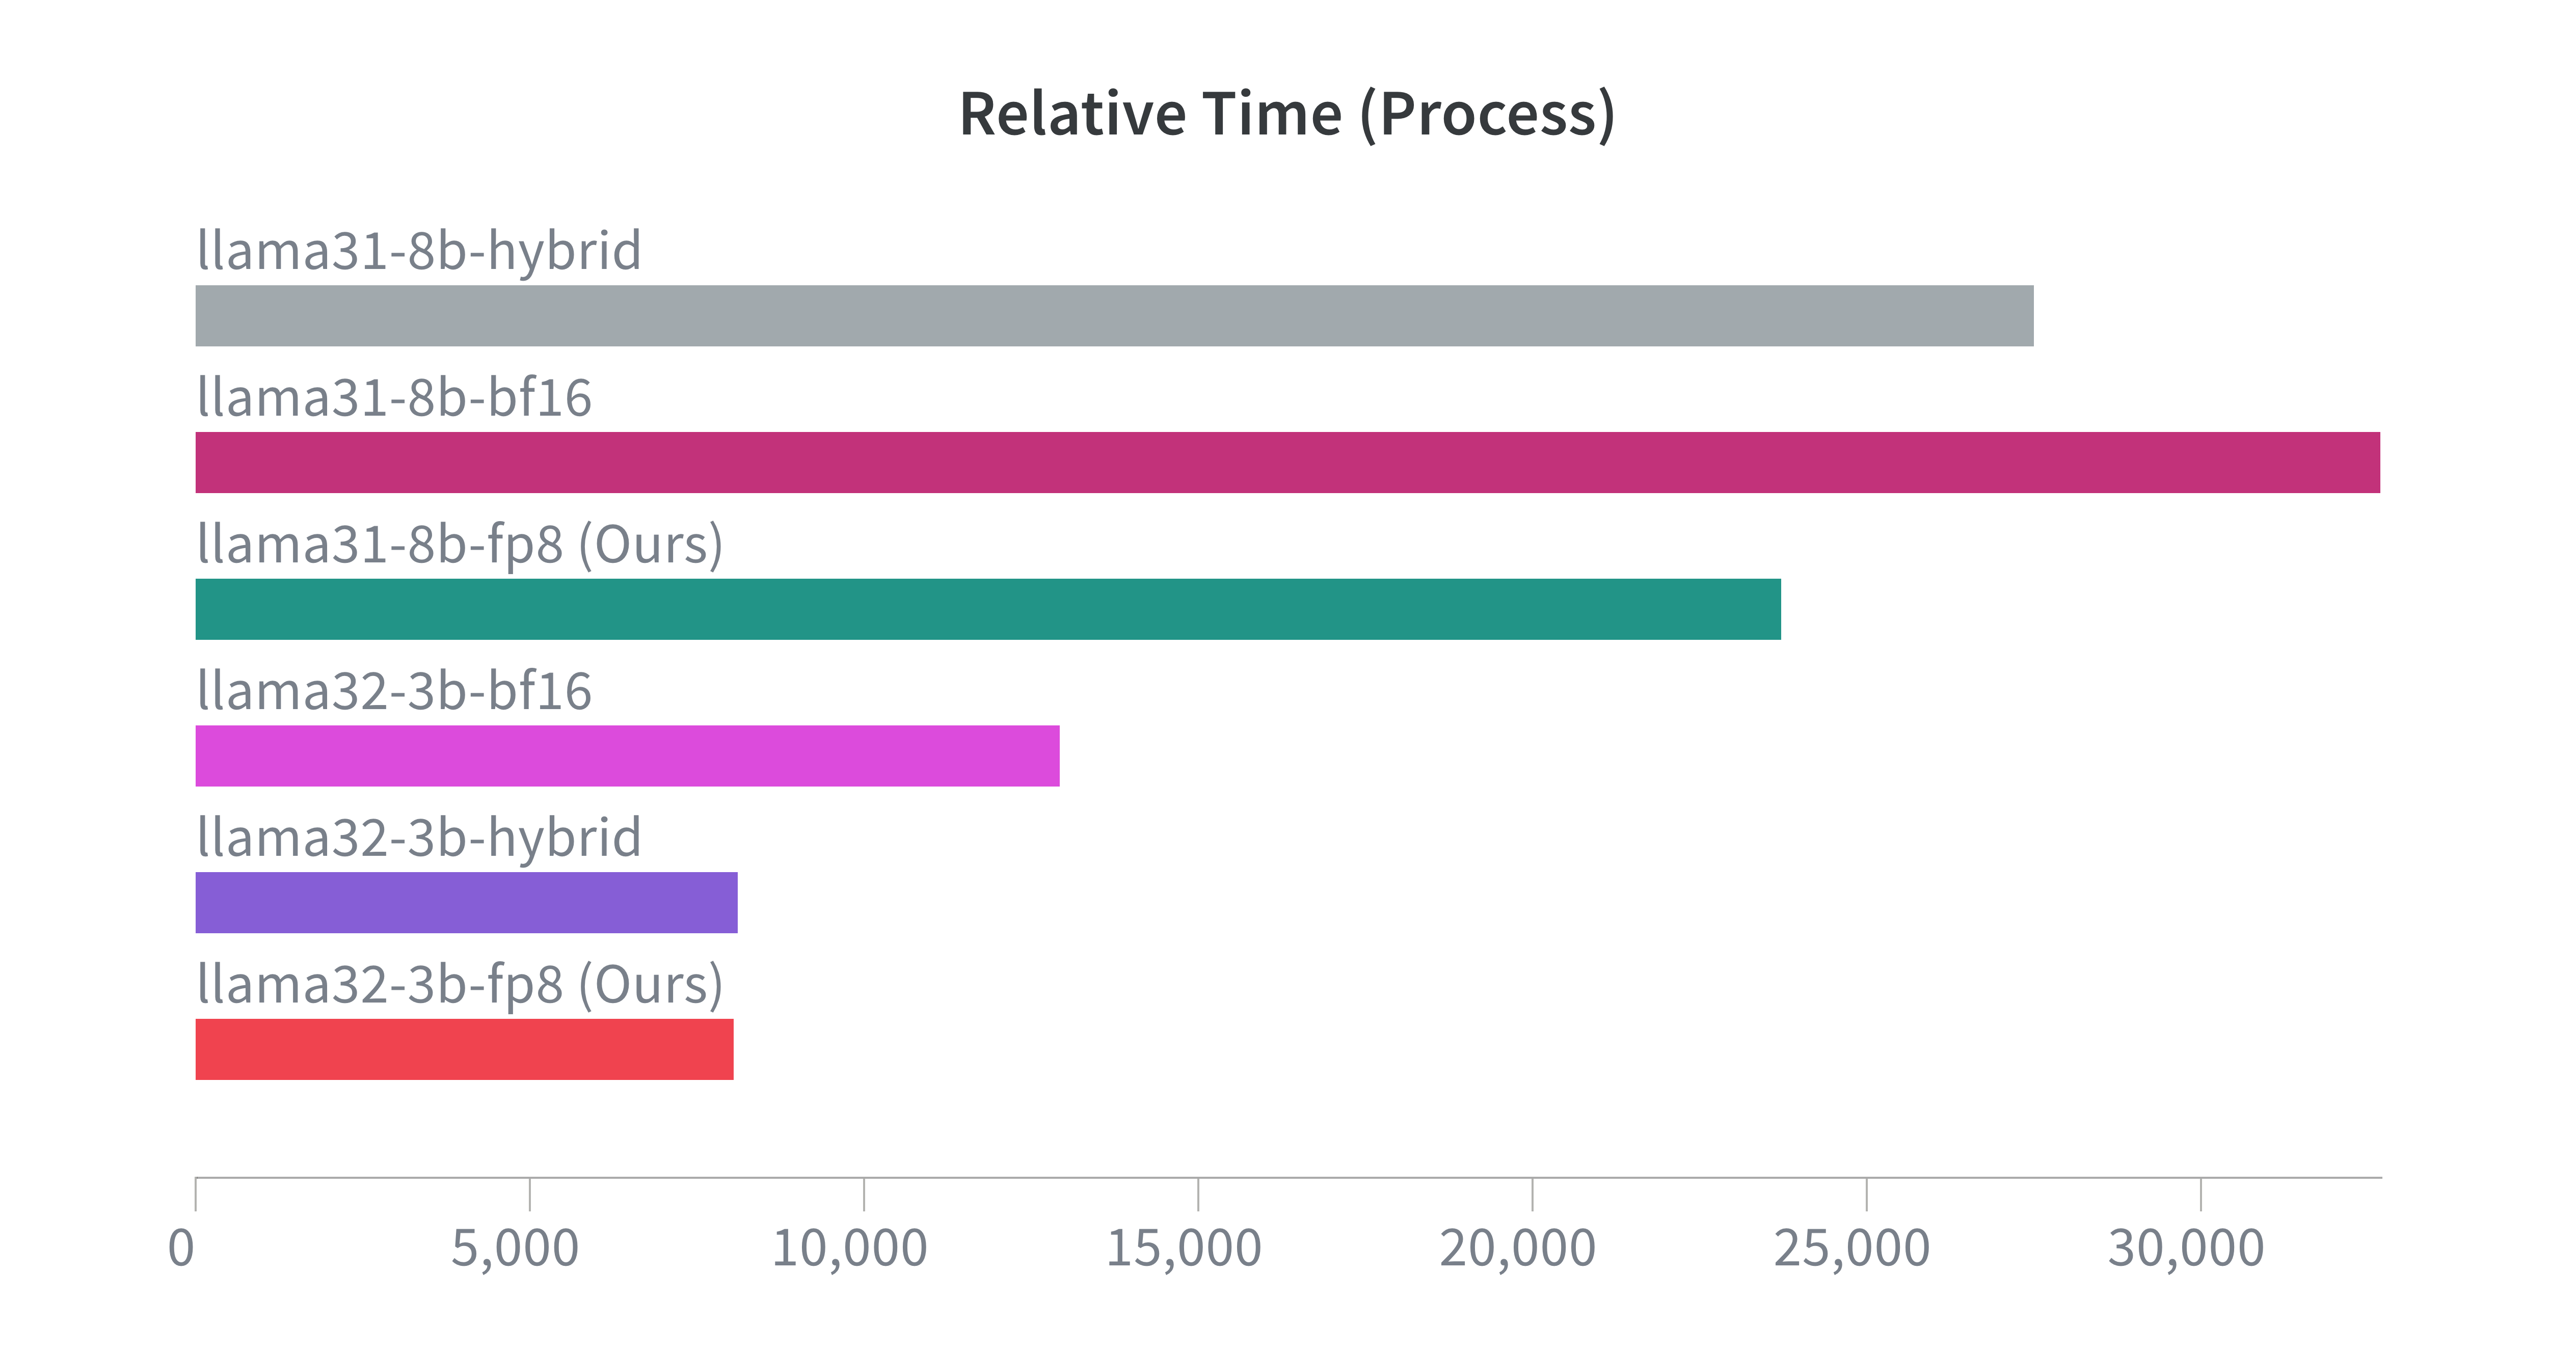
\includegraphics[width=0.9\linewidth]{figures/c4/training_time.png}
    \caption{Training time comparison across model configurations. Our layer-wise FP8 approach achieves substantial speedups, with the 3B model showing 42\% reduction (3.6h → 2.1h) and the 8B model demonstrating 27\% improvement over BF16 baseline.}
    \label{fig:training_time_comparison}
\end{figure}

For the 3B model, we achieve 42\% reduction in training time (3.6h → 2.1h) compared to BF16, closely matching the Hybrid FP8 baseline (2.2h). The performance advantage becomes more pronounced at the 8B scale, where our approach achieves 6.6 hours training time compared to 7.6 hours for Hybrid FP8 and 9.1 hours for BF16—representing a 27\% speedup over BF16 and 13\% improvement over Hybrid FP8.

\subsection{Numerical Stability Analysis}

A critical advantage of our layer-wise FP8 approach is exceptional numerical stability during training. Figure~\ref{fig:stability_comparison} illustrates loss variance across training steps, comparing our method against baseline approaches.

\begin{figure}[h]
    \centering
    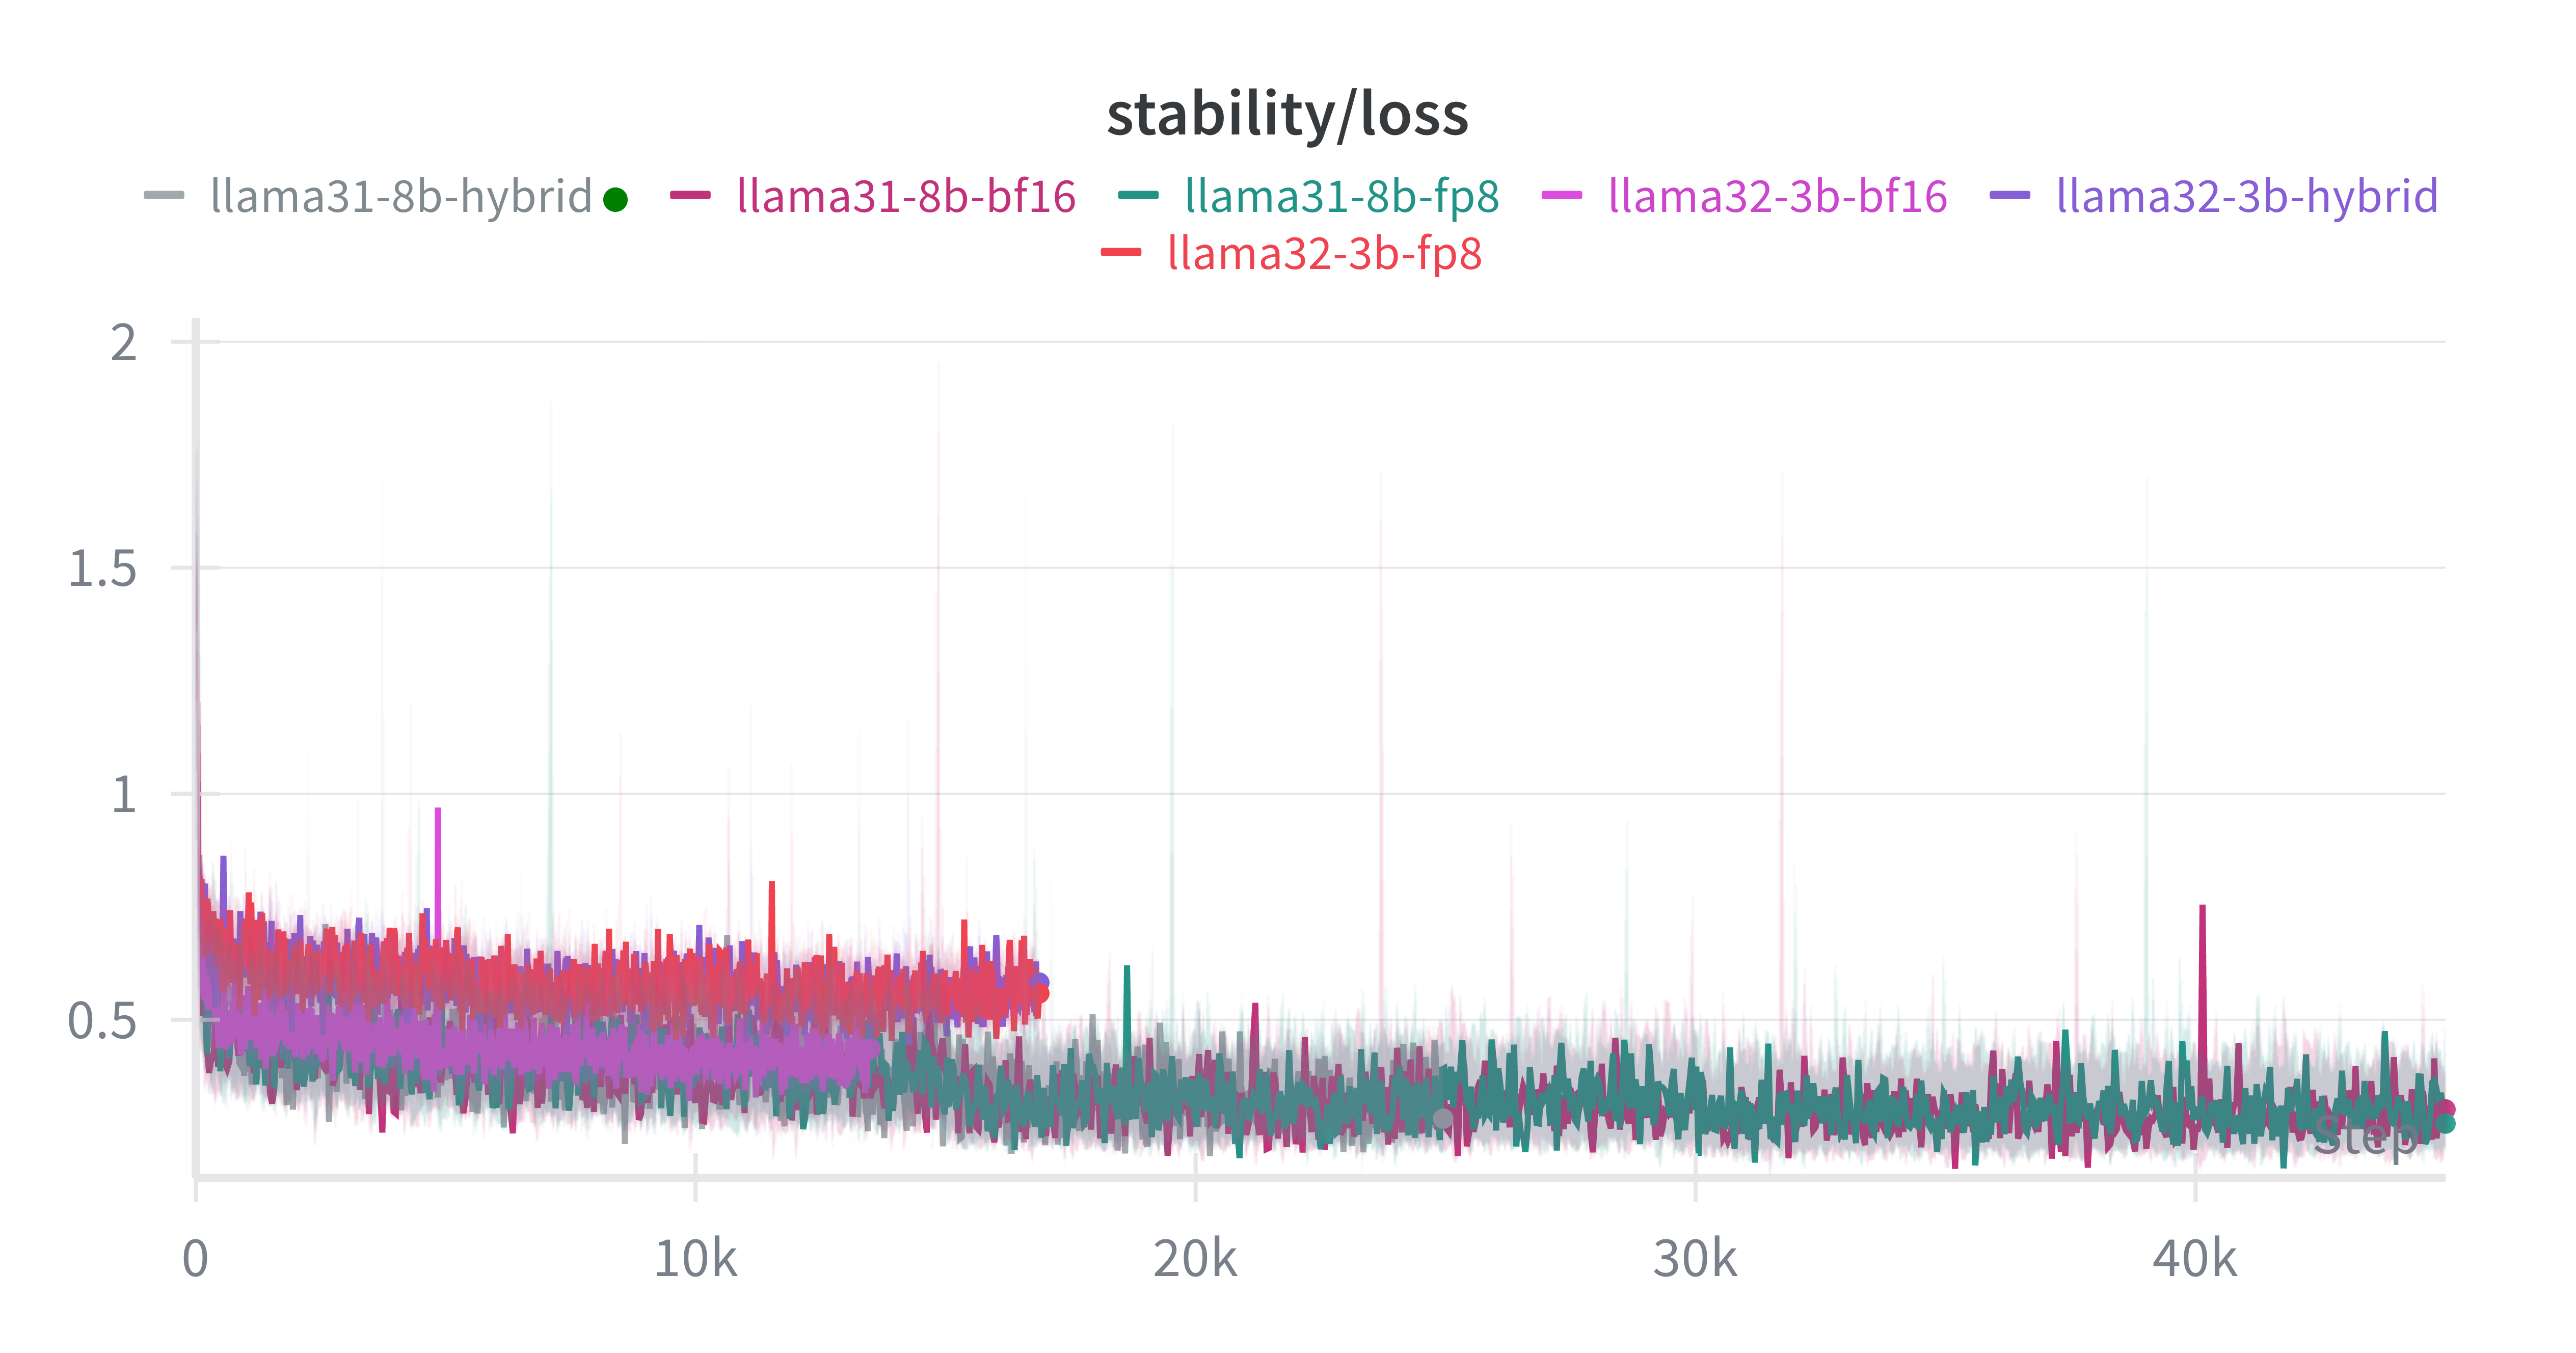
\includegraphics[width=0.9\linewidth]{figures/c4/numeric_stability.png}
    \caption{Numerical stability analysis showing loss variance over training steps. Our layer-wise FP8 approach (gray line) demonstrates exceptional stability with loss variance consistently below 0.4, significantly outperforming hybrid FP8 approaches which show periodic instability spikes reaching 0.8+ throughout training.}
    \label{fig:stability_comparison}
\end{figure}

Our selective use of E5M2 for high-dynamic-range operations (attention queries/keys) and E4M3 for stable operations (MLPs, values) results in superior numerical stability. The layer-wise FP8 approach maintains loss variance consistently below 0.4 throughout training, representing approximately 50\% lower variance compared to hybrid FP8 approaches that exhibit periodic instability spikes reaching 0.8 or higher.

This improved stability translates to more predictable training dynamics and reliable convergence, which is crucial for research reproducibility and model development. The lower variance indicates that our format assignment strategy effectively matches computational requirements with appropriate precision-range trade-offs for each component type.
